%% Exemplo de utilizacao do estilo de formatacao normas-utf-tex (http://normas-utf-tex.sourceforge.net)
%% Autores: Hugo Vieira Neto (hvieir@utfpr.edu.br)
%%          Diogo Rosa Kuiaski (diogo.kuiaski@gmail.com)
%% Colaboradores:
%%          Cézar M. Vargas Benitez <cesarvargasb@gmail.com>
%%          Marcos Talau <talau@users.sourceforge.net>


%\documentclass[openright]{normas-utf-tex} %openright = o capitulo comeca sempre em paginas impares
\documentclass[oneside]{normas-utf-tex} %oneside = para dissertacoes com numero de paginas menor que 100 (apenas frente da folha) 

\usepackage[alf,abnt-emphasize=bf,bibjustif,recuo=0cm, abnt-etal-cite=2, abnt-etal-list=99]{abntcite} %configuracao correta das referencias bibliograficas.

\usepackage[brazil]{babel} % pacote portugues brasileiro
\usepackage[utf8]{inputenc} % pacote para acentuacao direta
\usepackage{amsmath,amsfonts,amssymb} % pacote matematico
\usepackage{graphicx} % pacote grafico
\usepackage{times} % fonte times

%Podem utilizar GEOMETRY{...} para realizar pequenos ajustes das margens. Onde, left=esquerda, right=direita, top=superior, bottom=inferior. P.ex.:
%\geometry{left=3.0cm,right=1.5cm,top=4cm,bottom=1cm} 

% ---------- Preambulo ----------
\instituicao{Universidade Tecnol\'ogica Federal do Paran\'a} % nome da instituicao
\programa{Departamento Acadêmico de Eletrônica} % nome do programa
\area{Inform\'atica Industrial} % [Engenharia Biom\'edica] ou [Inform\'atica Industrial] ou [Telem\'atica]

\documento{Monografia} % [Disserta\c{c}\~ao] ou [Tese]
\nivel{Mestrado} % [Mestrado] ou [Doutorado]
\titulacao{Mestre} % [Mestre] ou [Doutor]

\titulo{\MakeUppercase{Robô Explorador de Ambientes}} % titulo do trabalho em portugues
\title{\MakeUppercase{Ambience Explorer Robot}} % titulo do trabalho em ingles

\autor{Luis Guilherme Machado Camargo} % autor do trabalho
\autordois{Marcelo Teider Lopes}
\autortres{Matheus Silva Araújo}
\cita{CAMARGO, Luis Guilherme M. ; LOPES, Marcelo Teider; ARAÚJO, Matheus Silva} % sobrenome (maiusculas), nome do autor do trabalho

\palavraschave{Palavra-chave 1, Palavra-chave 2, ...} % palavras-chave do trabalho
\keywords{Keyword 1, Keyword 2, ...} % palavras-chave do trabalho em ingles

%\comentario{\UTFPRdocumentodata\ apresentada ao \UTFPRdocumentodata\ da \ABNTinstituicaodata\ como requisito parcial para obten\c{c}\~ao do grau de ``\UTFPRtitulacaodata\ em Ci\^encias'' -- \'Area de Concentra\c{c}\~ao: \UTFPRareadata.}

\comentario{\UTFPRdocumentodata\ apresentada ao Departamento Acadêmico de Eletrônica da \ABNTinstituicaodata\ como requisito parcial para aprovação na Disciplina de Oficina de Integração 2.}


\orientador[Orientadora:]{Profa. Dra. Myriam Regattieri De Biase da Silva Delgado} % nome do orientador do trabalho
%\orientador[Orientadora:]{Nome da Orientadora} % <- no caso de orientadora, usar esta sintaxe
%\coorientador{Nome do Co-orientador} % nome do co-orientador do trabalho, caso exista
%\coorientador[Co-orientadora:]{Nome da Co-orientadora} % <- no caso de co-orientadora, usar esta sintaxe
%\coorientador[Co-orientadores:]{Nome do Co-orientador} % no caso de 2 co-orientadores, usar esta sintaxe
%\coorientadorb{Nome do Co-orientador 2}	% este comando inclui o nome do 2o co-orientador

\local{Curitiba} % cidade
\data{\the\year} % ano automatico


%---------- Inicio do Documento ----------
\begin{document}

\capa % geracao automatica da capa
\folhaderosto % geracao automatica da folha de rosto
%\termodeaprovacao % <- ainda a ser implementado corretamente

% dedicatória (opcional)
%\begin{dedicatoria}
%Texto da dedicat\'oria.
%\end{dedicatoria}

% agradecimentos (opcional)
\begin{agradecimentos}
Este trabalhado não teria sido possível sem o projeto anteriormente apresentado por Bruno Meneguele, Fernando Padilha e Vinicius Arcanjo.
Por emprestar o robô e pelos diversos esclarecimentos (muitas vezes sobre assuntos que não os envolviam) nosso muito obrigado.

À Professora Myriam nosso agradecimento por aceitar o desafio de nos orientar. 

Aos Professores Hugo Vieira e Mário Sérgio pela oportunidade sem par de aprendizado.
 
\end{agradecimentos}

% epigrafe (opcional)
%\begin{epigrafe}
%Texto da ep\'igrafe.
%\end{epigrafe}

%resumo
\begin{resumo}
Texto do resumo (m\'aximo de 500 palavras).
\end{resumo}

%abstract
\begin{abstract}
Abstract text (maximum of 500 words).
\end{abstract}

% listas (opcionais, mas recomenda-se a partir de 5 elementos)
\listadefiguras % geracao automatica da lista de figuras
\listadetabelas % geracao automatica da lista de tabelas
%\listadesiglas % geracao automatica da lista de siglas
%\listadesimbolos % geracao automatica da lista de simbolos

% sumario
\sumario % geracao automatica do sumario


%---------- Inicio do Texto ----------
% recomenda-se a escrita de cada capitulo em um arquivo texto separado (exemplo: intro.tex, fund.tex, exper.tex, concl.tex, etc.) e a posterior inclusao dos mesmos no mestre do documento utilizando o comando \input{}, da seguinte forma:
%\input{intro.tex}
%\input{fund.tex}
%\input{exper.tex}
%\input{concl.tex}


% ========== %
% INTRODUÇÃO %
% ========== %

\chapter{Introdução}

\section{Motivação}


\section{Objetivo}


\subsection{Objetivo Geral}


\subsection{Objetivos Específicos}


\section{Visão Geral do Projeto}


% ================ %
% SISTEMA MECÂNICO %
% ================ %

\chapter{Sistema Mecânico}

O robô utilizado no projeto é o mesmo robô construído durante o projeto \textbf{Robô Explorador de Labirintos 2D} \cite{RoboExplorador} desta mesma disciplina.

No projeto original o robô era utilizado para explorar e solucionar labirintos em duas dimensões feitos através de trilhas pretas em um chão branco, utilizado emissores e sensores de luz infravermelha para identificar a pista. 

Todo o projeto mecânico foi reutilizado neste trabalho, incluindo rodas, caixa de redução e chassi. Foram reutilizados também o sistema de alimentação e a uma placa \textit{Arduíno Duemilanove}; o conjunto de sensores do robô original foi substituído por uma câmera \textit{CMUCam3}.

\section{Projeto Mecânico}

O diagrama do projeto físico do robô é apresentado na Figura \ref{int_fig01}.

\begin{figure}[h!]
    \center
    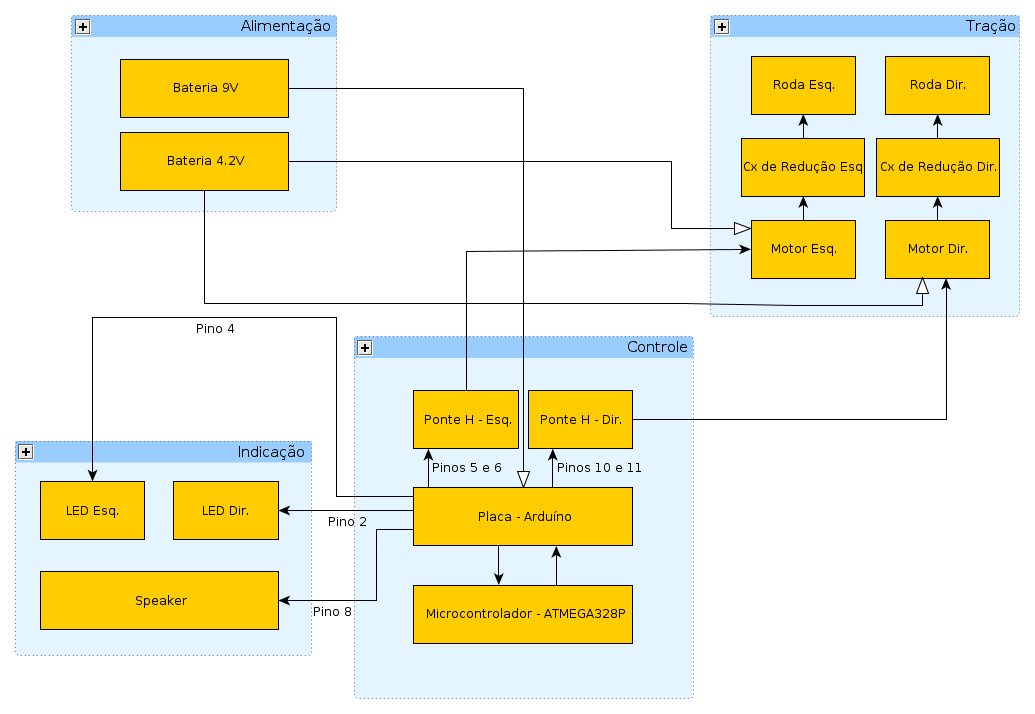
\includegraphics[scale=0.3]{imagens/robo.png}
    \caption{Diagrama do Robô}
    \label{int_fig01}
\end{figure}

\subsection{Sistema de Alimentação}

Conjunto de baterias utilizadas como alimentação do robô.

\subsubsection{Bateria de 9V}
Utilizada para alimentação do \textit{Arduíno Duemilanove}, uma bateria PP3.

\subsubsection{Bateria de 4,2V}
Usada na alimentação dos motores, bateria de câmera fotográfica digital.

\subsubsection{Bateria de 6V}
Usada na alimentação da CMUCam3, quatro pilhas AA em série.

\subsection{Sistema de Indicação}

LEDs e \textit{Speaker} usados para indicar as ações do robô.

\subsubsection{LEDs}
Usados para indicação dos estados do robô, detalhados na Tabela \ref{int_tbl01}

\begin{table}[h!]
    \centering
    \begin{tabular}{|c|c|c|} \hline
        \textbf{Estado} & \textbf{LED Esquerdo} & \textbf{LED Direito} \\ \hline
        Parado & Apagado & Apagado \\ \hline
        Andando para frente & Aceso & Apagado \\ \hline
        Virando para esquerda & Aceso & Apagado \\ \hline
        Virando para direita & Apagado & Aceso \\ \hline
    \end{tabular}
    \caption{Sistema de Indicação}
    \label{int_tbl01}
\end{table}

\subsubsection{Speaker}
Utilizado como indicador sonoro de estados específicos do sistema, como reconhecimento do objeto e início e fim da busca do mesmo.

\subsection{Sistema de Tração}

Para tração do robô foi construído um sistema baseado em um motor elétrico e duas rodas centrais.

\subsubsection{Motores}
Motor elétrico de corrente contínua \textit{Tamiya} de 3V com rotação de 12300 rpm, ou 205 voltas por segundo \cite{RoboExplorador}

\subsubsection{Caixas de redução}
Acopladas ao motor e às rodas reduzem a rotação do motor para que seja possível acionar as rodas. Na configuração usada, a redução é de 344:1 \cite{RoboExplorador}.

\subsubsection{Rodas}
O robô utiliza duas rodas \textit{off-road} em seu centro e uma esfera com giro livre atrás para manter o equilíbrio.

Com a rotação de 205 voltas/segundo e a redução de 344:1, a roda completa 0,6 voltas por segundo.

\subsection{Sistema de Controle}

Sistema para controle da movimentação do robô.

\subsubsection{Ponte H} 

A Ponte H é um circuito que permite a um microcontrolador acionar um motor de corrente contínua. Por questões eletrônicas \cite{RoboExplorador}, o circuito utilizado no projeto foi construído a partir de componentes discretos.

\subsubsection{Arduíno Duemilanove}

Placa \textit{Arduíno} utilizada no projeto anterior e reutilizada no projeto atual. Faz o interfaceamento dos diversos sistemas do projeto, \textit{i.e.}, recebe as decisões tomadas pelo Sistema de Navegação, embarcado na câmera, e aciona os motores para que o robô as execute. Seu funcionamento é detalhado na seção \ref{sec_arduino}.

\subsubsection{Microcontrolador ATMEGA328P}

Microcontolador presente da \textit{Arduíno Duemilanove}, os códigos construídos para controle do robô (Seção \ref{sec_soft_controle}) serão executados por ele.

\section{Plataforma Arduíno}
\label{sec_arduino}


\section{Software de Controle}
\label{sec_soft_controle}


% ======== %
% SENSORES %
% ======== %

\chapter{Sensores}

\section{Bússola}

\section{Câmera}


% ===== %
% VISÃO %
% ===== %

\chapter{Visão}

O sistema de visão, desenvolvido na \textit{CMUCam3}, é responsável principalmente por identificar e localizar o objeto a ser procurado no seu campo de visão, identificar objetos de interesse para serem utilizados na navegação, e identificar obstáculos. Ele também tem a função auxiliar de corrigir desvios na movimentação do robô. De forma a resolver esses problemas, diversas funcionalidades apresentadas pela \textit{CMUcam3} são utilizadas. Diversos exemplos e projetos já existentes também são aproveitados como referência.

\section{Identificação de objetos de interesse}

Uma das principais funções do sistema de visão é localizar, caso se encontre dentro de seu campo de visão, o objeto a ser procurado pelo robô. Como este é simples e possui uma única cor, de destaque, que não existe no ambiente proposto (e é improvável de se encontrar em um ambiente genérico) o mapa de cores obtido com a \textit{CMUcam} pode ser utilizado para localizar o objeto na imagem, aliado a uma ferramenta de reconhecimento de forma.

O sistema também deve localizar, dentro de seu campo de visão, objetos que se destaquem, para serem utilizados pelo sistema de navegação, de forma a identiicar a posição atual. Para a identificação desses objetos, ou pontos de interesse, as características de cor e forma também podem ser utilizadas. Técnicas adicionais para tornar o reconhecimento tolerável à rotação tridimensional não são necessárias, devido às informações obtidas pela bússola.

\section{Identificação de obstáculos}

Obstáculos podem ser identificados, na imagem, através do histograma da imagem obtida, ou então por detecção de bordas. A primeira abordagem é preferível por auxiliar a identificar as áreas (chão) por onde o robô pode se locomover, ao invés dos limites entre o chão e os obstáculos. A \ref{vis_fig01} apresenta algumas imagens exemplo obtidas no site da \textit{CMUcam3}.

\begin{figure}[h!]
    \center
    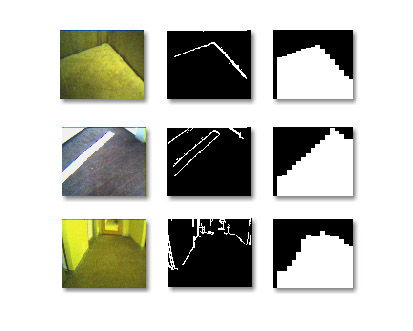
\includegraphics[scale=1]{imagens/polly_sample.jpg}
    \caption{Histograma e Detecção de Bordas de algumas imagens exemplo}
    \label{vis_fig01}
\end{figure}

\section{Correção de desvios}

De forma a corrigir eventuais desvios na movimentação do robô, causados por uma diferença de rotação entre as duas rodas, o sistema também deve identificar, na imagem, através da detecção de bordas e do mapa de cores, alguns objetos ou bordas de destaque, e caso saiam muito do lugar esperado para eles, corrigir sua rota.


% ========= %
% NAVEGAÇÃO %
% ========= %

\chapter{Navegação}

Para o robô encontrar o objeto anteriormente especificado ele deve saber se locomover dentro de um ambiente desconhecido. Para navegar no ambiente, o robô deve criar uma espécie de mapa que contenha informações que possibilitem sua locomoção no ambiente. Duas abordagens distintas são a representação de maneira global ou de maneira local [5].

De acordo com Jorg [5], a representação global procura descrever o ambiente da maneira mais fiel à realidade possível, indicando o mapa a partir de seus nodos e suas conexões, retendo o máximo de informação possível para conseguir manter uma consistência espacial global conforme o mapa vai sendo construído. A grande desvantagem da representação global é a necessidade de se reter e processar toda essa informação para criar-se o mapa, portanto conforme a quantidade de nodos aumenta, o mapa em si aumenta e a complexidade computacional também aumenta consideravelmente.

Na representação local os nodos (pontos de referência, denominados Place Agents) possuem informações apenas do próprio local, de quais são os nodos vizinhos, possíveis pontos de interesse (objetos de destaque para identificação do nodo, por exemplo) e informações pertinentes sobre como alcançar o próximo nodo (direção, existência de obstáculos, etc.) seja este nodo já presente no mapa ou não.

Para nosso projeto, a equipe optou por utilizar a representação local para o projeto, pois a abordagem global se torna ineficiente devido a sua complexidade computacional envolvida para manter a consistência do mapa. A abordagem local permite o escalonamento do sistema para permitir a ele operar em ambientes maiores.

\section{Construção do mapa}

Para a criação do mapa utilizamos principalmente a câmera CMUcam3 acoplada ao robô. A câmera é a principal responsável por adquirir informações do ambiente para a criação do mapa. Junto com a câmera, a bússola é utilizada para fornecer as direções entre um nodo e outro. Com as informações obtidas da câmera e da bússola, o robô deve ser capaz de construir um mapa do ambiente e deve ser capaz de locomover-se dentro do ambiente, procurando o objeto desejado e desviando de obstáculos caso necessário.

Inicialmente, ao ser inicializado num novo ambiente, o robô deve criar um nodo A que será demarcado como o primeiro nodo existente no mapa. A primeira informação a ser obtida será procurar características do ambiente ou objetos próximos ao nodo para caracterizar o nodo em questão. Após obter informações do ambiente atual, o robô deve observar seus arredores e definir outros nodos alcançáveis a partir do nodo atual. O robô então deve guardar informações pertinentes sobre como chegar a cada um dos nodos vizinhos, como direção e a existência de objetos de destaque. Tais informações sobre o caminho serão guardadas em ambos os nodos envolvidos (nodo A e nodo B, inicio e destino, respectivamente). Dentre todos os nodos vizinhos, o sistema escolhe um e se locomove até ele. O processo então é repetido diversas vezes até que o mapa seja completamente montado (não existe nenhum nodo alcançável não visitado) ou o objeto seja encontrado.

\section{Roteamento}

Na representação local os nodos (pontos de referência, denominados Place Agents) possuem informações apenas do próprio local, de quais são os nodos vizinhos, possíveis pontos de interesse (objetos de destaque para identificação do nodo, por exemplo) e informações pertinentes sobre como alcançar o próximo nodo (direção, existência de obstáculos, etc.) seja este já presente no mapa ou não. Na representação local, para se alcançar um nodo já mapeado e que não seja vizinho ao atual será necessário um algoritmo de roteamento no sistema, onde cada Place Agent pergunta por essa informação aos seus vizinhos e assim sucessivamente até que o nodo requisitado seja encontrado.

Quando o nodo requisitado é encontrado o robô traça um caminho para chegar ao local desejado, passando por nodos já existentes. 


% ========= %
% CONCLUSÃO %
% ========= %

\chapter{Conclusão}

No atual momento do projeto, a comunicação entre \textit{CMUcam3} e \textit{Arduíno} ainda não foi implementada, por esse motivo ainda não foi possível fazer os testes de exploração e identificação do objeto.

Analisando a estrutura do robô desde a parte mecânica, eletrônica e as estratégias para exploração e localização do objeto encontrado, espera-se que o robô consiga encontrar um objeto especifico e de destaque dentro de um ambiente pequeno, com as dimensões 168,2 cm por 118,9 cm.

Espera-se também conseguir implementar corretamente um código de exploração inteligente baseado em representações locais para locomoção do robô dentro do espaço determinado. Além disso, conseguir aplicar um código para reconhecer o objeto a ser encontrado utilizando características de destaque (cores fortes, forma, etc.) do objeto. Tais características do robô (locomoção e identificação) serão controladas pela câmera acoplada ao robô, a \textit{CMUcam3}.

Como continuação deste projeto, seria interessante ver o robô se locomovendo em espaços maiores e mais dinâmicos e também que o robô possa identificar objetos mais familiares ao dia a dia como algum equipamento ou molho de chaves.


%---------- Referencias ----------
\bibliography{reflatex} % geracao automatica das referencias a partir do arquivo reflatex.bib

%---------- Apendices (opcionais) ----------
\apendice

\chapter{Caderno de Bordo}

%\chapter{Nome do Ap\^endice}

%Use o comando {\ttfamily \textbackslash apendice} e depois comandos {\ttfamily \textbackslash chapter\{\}}
%para gerar t\'itulos de ap\^en-dices.


% ---------- Anexos (opcionais) ----------
%\anexo
%\chapter{Nome do Anexo}

%Use o comando {\ttfamily \textbackslash anexo} e depois comandos {\ttfamily \textbackslash chapter\{\}}
%para gerar t\'itulos de anexos.


% --------- Lista de siglas --------
%\textbf{* Observa\c{c}\~oes:} a lista de siglas nao realiza a ordenacao das siglas em ordem alfabetica
% Em breve isso sera implementado, enquanto isso:
%\textbf{Sugest\~ao:} crie outro arquivo .tex para siglas e utilize o comando \sigla{sigla}{descri\c{c}\~ao}.
%Para incluir este arquivo no final do arquivo, utilize o comando \input{arquivo.tex}.
%Assim, Todas as siglas serao geradas na ultima pagina. Entao, devera excluir a ultima pagina da versao final do arquivo
% PDF do seu documento.


%-------- Citacoes ---------
% - Utilize o comando \citeonline{...} para citacoes com o seguinte formato: Autor et al. (2011).
% Este tipo de formato eh utilizado no comeco do paragrafo. P.ex.: \citeonline{autor2011}

% - Utilize o comando \cite{...} para citacoeses no meio ou final do paragrafo. P.ex.: \cite{autor2011}



%-------- Titulos com nomes cientificos (titulo, capitulos e secoes) ----------
% Regra para escrita de nomes cientificos:
% Os nomes devem ser escritos em italico, 
%a primeira letra do primeiro nome deve ser em maiusculo e o restante em minusculo (inclusive a primeira letra do segundo nome).
% VEJA os exemplos abaixo.
% 
% 1) voce nao quer que a secao fique com uppercase (caixa alta) automaticamente:
%\section[nouppercase]{\MakeUppercase{Estudo dos efeitos da radiacao ultravioleta C e TFD em celulas de} {\textit{Saccharomyces boulardii}}
%
% 2) por padrao os cases (maiusculas/minuscula) sao ajustados automaticamente, voce nao precisa usar makeuppercase e afins.
% \section{Introducao} % a introducao sera posta no texto como INTRODUCAO, automaticamente, como a norma indica.


\end{document}
